%%%% ijcai21.tex

\typeout{IJCAI--21 Instructions for Authors}

% These are the instructions for authors for IJCAI-21.

\documentclass{article}
\pdfpagewidth=8.5in
\pdfpageheight=11in
% The file ijcai21.sty is NOT the same than previous years'
\usepackage{ijcai21}

% Use the postscript times font!
\usepackage{times}
\usepackage{soul}
\usepackage{url}
\usepackage[hidelinks]{hyperref}
\usepackage[utf8]{inputenc}
\usepackage[small]{caption}
\usepackage{graphicx}
\usepackage{amsmath}
\usepackage{amsfonts}
\usepackage{amsthm}
\usepackage{booktabs}
\usepackage{algorithm}
\usepackage{algorithmic}
\urlstyle{same}
\usepackage[export]{adjustbox}

%%%%%%%%%%%%%%%%%%%%%%%%%%%   MACROS   %%%%%%%%%%%%%%%%%%%%%%%%%%%%%%%%%

\newcommand{\xmu}[2]{x_{#1_#2}^{#2}(t)}
\newcommand{\xnotmu}[2]{x_{#1_#2}^{#2}}
\newcommand{\xmudash}[2]{x_{#1_#2}^{#2}(t')}
\newcommand{\payoff}[2]{P^{#2}_{#1_#2, #1_{-#2}}}

\newcommand{\dxmu}[1]{\dot{x}_{#1_\mu}^{\mu} (t)}
\newcommand{\dnotxmu}[1]{\dot{x}_{#1_\mu}^{\mu}}
\newcommand{\hxmu}[1]{\hat{x}_{#1_\mu}^{\mu} (t)}
\newcommand{\hnotxmu}[1]{\hat{x}_{#1_\mu}^{\mu}}
\newcommand{\hxnu}[1]{\hat{x}_{#1_\nu}^{\nu} (t)}
\newcommand{\hxmudash}[1]{\hat{x}_{#1_\mu}^{\mu} (t')}
\newcommand{\hxnudash}[1]{\hat{x}_{#1_\nu}^{\nu} (t')}

\newcommand{\txmu}[2]{\tilde{x}_{#1_#2}^{#2}(t)}
\newcommand{\dtxmu}[2]{\dot{\tilde{x}}_{#1_#2}^{#2}(t)}
\newcommand{\tpayoff}[2]{\tilde{P}^{#2}_{#1_#2, #1_{-#2}}}
\newcommand{\talpha}{\tilde{\alpha}}
\newcommand{\ttau}{\tilde{\tau}}
\newcommand{\htau}{\hat{\tau}}
\newcommand{\xfixed}{x_\infty}
\newcommand{\ezerof}{\eta_{0, \infty}}
\newcommand{\eonef}{\eta_{1, \infty}}

\newcommand{\xpert}{\hat{x}(t)}
\newcommand{\xpertdash}{\hat{x}(t')}
\newcommand{\ezeropert}{\hat{\eta}_0(t)}
\newcommand{\eonepert}{\hat{\eta}_1(t)}

\newcommand{\eom}{\frac{\dxmu{i}}{\xmu{i}{\mu}} - \alpha \ttau \left ( \sum_{i_{-\mu}} \payoff{i}{\mu} \prod_{\kappa \neq \mu} \xmu{i}{\kappa} \right ) + \\ \alpha \htau \left ( \frac{1}{\sqrt{N}} \sum_{i_\mu i_{-\mu}} \xmu{i}{\mu} \payoff{i}{\mu} \prod_{\kappa \neq \mu} \xmu{i}{\kappa} \right ) - \talpha \rho^{\mu}_{i}(t)}

\usepackage{xcolor} % REMOVE THIS AT THE END
\newcommand\fb[1]{\textcolor{blue}{FB: #1}}
\newcommand\ah[1]{\textcolor{red}{AH: #1}}
%%%%%%%%%%%%%%%%%%%%%%%%%%%%%%%%%%%%%%%%%%%%%%%%%%%%%%%%%%%%%%%%%%%%%%%%

% the following package is optional:
%\usepackage{latexsym}

% See https://www.overleaf.com/learn/latex/theorems_and_proofs
% for a nice explanation of how to define new theorems, but keep
% in mind that the amsthm package is already included in this
% template and that you must *not* alter the styling.
\newtheorem{example}{Example}
\newtheorem{theorem}{Theorem}

% Following comment is from ijcai97-submit.tex:
% The preparation of these files was supported by Schlumberger Palo Alto
% Research, AT\&T Bell Laboratories, and Morgan Kaufmann Publishers.
% Shirley Jowell, of Morgan Kaufmann Publishers, and Peter F.
% Patel-Schneider, of AT\&T Bell Laboratories collaborated on their
% preparation.

% These instructions can be modified and used in other conferences as long
% as credit to the authors and supporting agencies is retained, this notice
% is not changed, and further modification or reuse is not restricted.
% Neither Shirley Jowell nor Peter F. Patel-Schneider can be listed as
% contacts for providing assistance without their prior permission.

% To use for other conferences, change references to files and the
% conference appropriate and use other authors, contacts, publishers, and
% organizations.
% Also change the deadline and address for returning papers and the length and
% page charge instructions.
% Put where the files are available in the appropriate places.

%PDF Info Is REQUIRED.
\pdfinfo{
/TemplateVersion (IJCAI.2021.0)
}

\title{Stability and Chaos in Multi-Agent Reinforcement Learning}

% Single author syntax
\author{Submission number 3289
%Aamal Hussain$^1$\footnote{Contact Author}\And
%Francesco Belardinelli$^1$\\
%\affiliations
%$^1$Imperial College London\\
%\emails
%\{aamal.hussain15, francesco.belardinelli\}@imperial.ac.uk,
}

\begin{document}

\maketitle

\begin{abstract}

Modelling the dynamics of Q-Learning is an active and important topic for the sake of developing an \textit{a priori} understanding of multi-agent reinforcement learning. In this paper, we apply methods from evolutionary game theory to analyse the stability of Q-Learning in $p$-player games with generalised payoff matrices. We determine the effect that the number of players, payoff correlations, and agent parameters have on the likelihood that the system converges to a stable fixed point, as opposed to displaying unstable behaviour. 
%
This study allows for parameters to be appropriately chosen to ensure the safe convergence of a learning algorithm and as a first step towards understanding the range of behaviours that can be displayed by 
%learning 
using Q-learning. We validate our theoretical results through numerical simulations and show that, within the bounds of experimental error, the region of instability can be characterised by the learning dynamics.

\end{abstract}

\section{Introduction}
%%%%%%%%%%%%% INTRO %%%%%%%%%%%%%%%%%%%%%

\label{sec::Intro}

Single-agent reinforcement learning (RL) is a well-established
framework for allowing agents to learn optimal strategies when trained
on an iterated task \cite{Sutton2018}. For the realisation of complex tasks,
such as air traffic control, market negotiations, and multi-robot
coordination, however, it is required that the system be modelled as a
multi-agent system (MAS). Such systems are less well-understood, since a given agent is tasked with
optimising a reward function that depends not only on a,
non-stationary environment, but also on the actions of other, possibly
loosely coupled, agents \cite{schwartz:reinforcement}.

It is, therefore, of paramount importance to develop a strong
theoretical understanding of multi-agent reinforcement learning (MARL)
to allow an \textit{a priori} understanding of the behaviour of a given
learning algorithm. Fortunately, the study of MAS is not unique to the
field of AI and has been extensively investigated from the point of view of
economics and game theory as well
\cite{shoham_leyton-brown_2008,leslie:iql}. In particular,
evolutionary game theory (EGT) considers the problem of a MAS that is
repeatedly exposed to an iterated game. This idea shares a strong
resemblance with MARL and, in fact, in \cite{tuyls:iteratedgames} it was
shown that techniques from EGT may be fruitfully applied to the analysis of
Q-Learning.

An important result in modelling multi-agent systems from the EGT
perspective is that, when games are learnt and the assumptions of
rationality and perfect information are lifted, games may not converge
to an equilibrium. Instead, as shown in \cite{sanders:prevalence}, the
dynamics may be more complex and even chaotic \cite{strogatz:2000}. In fact, chaotic behaviour has been found in a wide range of learning algorithms \cite{svs:fp,piliouras:chaoticmaps} The present work further
describes to what extent the emergence of such behaviours depends on the
parameters of the games and the learning algorithm. 

\paragraph{Contribution}
In this study, we will be considering the question: how does the likelihood of convergent behaviour, as opposed to instability, depend on the parameters of a homogeneous multi-agent system which is trained on an iterated normal-form game using Q-learning?
In investigating this
question, we will make the following assumptions:
%
%\begin{enumerate}
    %\item
    (1) There is a finite set of agents, though its size $p$ can be
      arbitrarily large.
    %\item 
    (2) The agents (sometimes referred to as players) have a discrete strategy space.
%
%  \item 
(3) The agents  are homogeneous, i.e., they all share the same parameters. 
%    
%\end{enumerate}

We find that our analysis gives a strong indication for how the stability of learning depends on its parameters, and that these predictions are confirmed in experiments. Specifically, we find that unstable dynamics become more prominent as the parameters \textit{step length}
$\alpha$ and \textit{intensity of choice} $\tau$  of
Q-learning increase. By comparison, the
correlation $\Gamma$ between payoffs, which measures how cooperative or competitive a game is, has a negligible affect on stability. In addition, we find that regardless of the choice of these
parameters, the likelihood of unstable behaviours increases monotonically with the number of players $p$.

%%%%%%%%%%%%% END INTRO %%%%%%%%%%%%%%%%%%%%%

%%%%%%%%%%%%% LIT REVIEW %%%%%%%%%%%%%%%%%%%%%

\paragraph{Related Work}
The theory of evolutionary game dynamics \cite{von-Neumann:games}
considers game-like settings in which agents repeatedly interact
with one another (i.e., `iterated games'). The outcome of these interactions depends on a payoff
matrix; `strong' strategies which maximise the reward are promoted,
whilst `weaker' strategies diminish. The \textit{replicator dynamic}
models this behaviour as a differential equation, and allows one to determine whether, after a
number of iterations, the game is likely to converge to some fixed
equilibrium \cite{shoham_leyton-brown_2008}.

Iterated games are considered imperfect, in that agents make decisions by attempting to anticipate and respond to their opponents' behaviour
based on experience \cite{galla:cycles}. 

In such games \cite{galla:complex}, it is found that cycles, as well as more complex behaviours, can emerge when two agents play using the \textit{experience weighted attraction} (EWA) learning algorithm \cite{hocamerer:ewa}. A rigorous theoretical analysis of EWA, results in a method for characterising how complex dynamics, such as chaos or cycles, depends on the game parameters. \cite{sanders:prevalence} extends this analysis to generic $p$-player games, and show that chaotic
dynamics are more likely to be observed as the number $p$ of players
increases.

It is evident, therefore, that in the case of learning on iterated
games, convergence to stable equilibria cannot be taken for granted. It would therefore be fruitful to bring these
analyses from EGT to better understand reinforcement learning from an
AI perspective.

In \cite{tuyls:iteratedgames}, the authors derive a continuous time deterministic approximation of  Q-Learning
and show its relation to the replicator
dynamic. In doing so, they present a dynamical system that
has been used to accurately analyse the behaviour of Q-Learning \cite{bloembergen:survey}. One such analysis is \cite{piliouras:catastrophe} which analyses a variant of the Q-Learning dynamics. The authors show that changes in the exploration parameter (here called the `intensity of choice' $\tau$) can lead to different qualitative behaviours. Their study shares the same general conclusions as our own, though through a different methodology. In addition, we aim also to characterise how the number $p$ of players  and the agent memory $\alpha$ affect the behaviour of Q-learning.

%%%%%%%%%%%%% END LIT REVIEW %%%%%%%%%%%%%%%%%%%%%


%%%%%%%%%%%%% PRELIMS %%%%%%%%%%%%%%%%%%%%%

\section{Background on Q-learning}

%Before presenting the technical arguments of this study, 
We now provide the specifics of the types of games and algorithm that we analyse in the subsequent sections.
%
We consider \textit{normal form games} consisting of: a finite set of players, with individual action spaces $\mathcal{A}$ (though we assume that all players share the same strategy space), and payoff functions for each player. The agents choose an action from their strategy space and receive a reward from their payoff matrix depending on the actions of all players. The payoffs remain unchanged across iterations. Examples of these normal form games include the popular Prisoner's Dilemma or Matching Pennies games \cite{tuyls:iteratedgames}.

The Q-learning approach requires
an agent to choose an action $i \in \mathcal{A}$ at step $k$ with probability
%
\begin{equation}
    x_i(k) = \frac{e^{\tau Q_i(k)}}{\sum_j e^{\tau Q_j(k)}}
\end{equation}
%
where $\tau \in [0, \infty)$ is the \textit{intensity of choice} as described at the end of this section, and $Q_i$ denotes the \textit{Q-value} of an action $i$, which is to be updated at each step according to
%
\begin{equation}
\label{eqn::Qupdate}
    Q_i(k+1) = (1 - \alpha) Q_i(k) + \alpha (r + \gamma \max_j Q_j(k))
\end{equation}
%
where $\alpha \in [0, 1]$ is the \textit{step length} parameter described below, $r$ is the immediate reward received, and $\gamma \in [0, 1]$ is the discount factor. Note we use the terms `payoff' and `reward' interchangeably.

By analysing this algorithm, Tuyls et al. derive a continuous-time, deterministic model of Q-learning, and verify empirically its accuracy. This model (which can be found in \cite{tuyls:iteratedgames} and is reproduced in the supplementary material Sec~S2.1 for completeness) 
makes it clear that the long term strategy selection of the agents is dependent on parameters $\alpha$ and $\tau$, as well as the payoffs themselves. In this study, therefore, we aim to establish the nature of this dependence. Specifically, the parameters we consider are:

%\begin{enumerate}
1.~The \textit{step length} $\alpha \in [0, 1]$. Low values of $\alpha$ denote smaller
    updates. Heuristically, we can consider this to be the memory of the agent: lower $\alpha$
    denotes longer memory.
    
2.~The \textit{intensity of choice} $\tau \in [0, \infty)$,
%as
%      termed by Sanders et al.  \cite{Sanders2018}. This 
which is sometimes
      written as $\beta$ in the literature \cite{piliouras:catastrophe}.  $\tau =
      0$ results in all actions being selected with equal probability,
      regardless of their Q-value, whilst $\tau \rightarrow \infty$
      results in the action with the highest Q-value chosen at every
      step. 
    
3.~The \textit{payoff
      correlation} $\Gamma \in [-1, p-1]$. Since there are an infinite number of realisations
      of the payoff matrices, we parameterise the payoffs by their correlations. To do this, we assume
      that the payoff matrices are drawn from a multi-variate Gaussian
      with mean zero and covariance matrix parameterised by
      $\Gamma$.In the subsequent sections, we will take an average over this Gaussian to determine the expected behaviour a MAS will take where the payoffs have a particular choice of $\Gamma$. $\Gamma = -1$
      indicates a zero-sum game, in which the sum of payoffs for a
      given action across all agents is zero, resulting in a purely
      competitive game. $\Gamma = p-1$ indicates a purely cooperative game
      in which all agents share the same payoffs. The manner in which
      a game is generated from the choice of $\Gamma$ is described in
      (\ref{eqn::Payoffs}) and follows the same procedure as
      outlined in \cite{sanders:prevalence}.
%\end{enumerate}

%%%%%%%%%%%%% THEORY %%%%%%%%%%%%%%%%%%%%%

\section{Stability Analysis of Q-Learning} \label{sec::Theory}

In this section, we determine how the choice of parameters
$\alpha$ and $\tau$, alongside the choice of payoff matrix and the number $p$ of players affects the
stability of the continuous-time model of Q-learning. As the values in the
payoff matrices can take any real number, however, there is an infinite number
of possible realisations of games. Of course, it would not be possible
to analyse every possible game, so we instead follow the procedure
outlined in \cite{coolen:minority,galla:complex} to average over
these realisations (Sec \ref{sec::eff_dyn}). This yields the \textit{effective
dynamics}, the dynamics averaged over all realisations of payoff
matrices. Then, in Sec \ref{sec::stability}, we perform a linear stability analysis on these dynamics around
equilibrium points to determine the conditions under which a fixed
point is stable. As this process is complex, we focus on the main steps in this paper, and refer to the supplementary material for the technical details. Sections from the Supplementary Material are denoted with the prefix S.

\subsection{Generalised Dynamics}
\label{sec::gen_dyn}

Our first point of call is to write  the dynamics of Tuyls et al. for a general $p$-player
game. This yields the dynamics (\ref{eqn::pEOM}), where player $\mu$
chooses action $i_{\mu}$ from its strategy space $\mathcal{A}$ at time
$t$ with probability $\xmu{i}{\mu}$ and receives a reward
$\payoff{i}{\mu}$ from its payoff matrix $P^\mu$ depending on its own
action and the actions of all other agents $i_{-\mu}$, where $i_{-\mu}$ denotes the set $\{ i_\kappa : \kappa \in \{1, 2,
\ldots , p\} \setminus \{\mu\} \}$ and $-i_{\mu}$ denotes the set
$\mathcal{A} \setminus {i_\mu}$.
%
\begin{eqnarray}
\label{eqn::pEOM}
%\begin{split}
    \frac{\dot{\xmu{i}{\mu}}}{\xmu{i}{\mu}} = \alpha \tau \big( \sum_{i_{-\mu}} \payoff{i}{\mu} \prod_{\kappa \neq \mu} \xmu{i}{\kappa} - \\
    \sum_{i_\mu i_{-\mu}} \xmu{i}{\mu} \payoff{i}{\mu} \prod_{\kappa \neq \mu} \xmu{i}{\kappa} \big) + \alpha \sum_{j_\mu \in -i_\mu} \xmu{j}{\mu} ln \frac{\xmu{j}{\mu}}{\xmu{i}{\mu}}    \nonumber
%\end{split}
\end{eqnarray}

For the sake of brevity, we sometimes drop the explicit dependence on $t$ in the notation of $\xmu{i}{\mu}$, and allow it to be inferred.

To average over all payoff elements , we assert that they
are generated by a multi-variate Gaussian distribution
with mean zero and covariance given as
%
\begin{equation}
\label{eqn::Payoffs}
%    \begin{split}
        \mathbb{E}\left [ \payoff{i}{\mu} \payoff{i}{\nu} \right] = \begin{cases}
        \frac{1}{N^{p-1}} &  \text{ if } \nu = \mu \\
        \frac{\Gamma}{(p-1) N^{p-1}} & \text{ otherwise. }
        \end{cases}
%    \end{split}
\end{equation}

The motivation for choosing a
Gaussian distribution is to allow for the use of Gaussian identities when
determining the average \cite{Zinn-Justin:QFT}. Furthermore, the domain of the multi-variate Gaussian is over all possible realisations of the payoff elements (i.e., over $\mathbb{R}^{p \cdot N^p}$). This means that we can accurately consider any set of payoff matrices to be drawn from a Gaussian. 

\subsection{The Effective Dynamics}
\label{sec::eff_dyn}


Our aim is first find to the corollary of (\ref{eqn::pEOM}) for the case of averaged payoff elements, we call this the `effective dynamics'. In order to find these dynamics we take a similar approach to that outlined in \cite{mezard:spinglass}. The idea is as follows. We first take a path integral over the entire trajectory as the \textit{generating functional} $Z$. This gives a single value which can be assigned to the trajectory. We can then find an expression for the expected value of $Z$ by averaging over all payoff elements, giving $\mathbb{E}[Z]$. Finally, we notice that, in the same way that $Z$ was generated from an equation of motion, so $\mathbb{E}[Z]$ may be considered as generated from an `averaged' equation of motion, which we call the \textit{effective dynamics}. These dynamics, then, form the required average case of (\ref{eqn::pEOM}).

The generating functional of the dynamics (\ref{eqn::pEOM}) is given as

{\small
\begin{equation}
\label{eqn::separatePayoffs}
  \begin{split}
  Z(\Vec{\psi}) = \int D[\Vec{x}, \Vec{\hat{x}}] exp( i \sum_{i, \mu} \int dt [ \hnotxmu{i} (\frac{\dnotxmu{i}}{\xnotmu{i}{\mu}} - \talpha \rho_i^\mu (t) - h_i^\mu (t))]) \\ \times  exp(-i \alpha \ttau \sum_{\mu} \sum_{i_\mu, i_{-\mu}} \int dt [\hnotxmu{i} \payoff{i}{\mu} \prod_{\kappa \neq \mu} \xnotmu{i}{\kappa} )])) 
    \\ \times  exp(-i \alpha \ttau \sum_{\mu} \sum_{j_\mu, i_\mu, i_{-\mu}} \int dt [\hnotxmu{j}  \xnotmu{i}{\mu} \payoff{i}{\mu} \prod_{\kappa \neq \mu} \xnotmu{i}{\kappa}])) 
  \\ \times exp(i \sum_{i, \mu}
  \int dt[\xnotmu{i}{\mu} \psi^\mu_i(t)]),
\end{split}
\end{equation}
}

where $\Vec{\psi_i(t)}$ and
$\Vec{\phi_i(t)}$ generate the necessary correlation functions. These act simply as a mathematical tool and will be set to zero at the end of the calculation \cite{coolen:minority}. 

The last two exponentials contain the payoff elements of the game. These are randomly generated using a multi-variate gaussian and then held fixed for the rest of the game. We employ the mean and covariance expressions given in (\ref{eqn::Payoffs}) to average over all possible realisations of these elements. This gives us a new form for an averaged generating functional. The technical details of how this averaging is performed is given in the supplementary material (Sec~S2.3-S2.5). 

As mentioned, in the same way that (\ref{eqn::pEOM}) gives rise to the functional $Z(\Vec{\psi})$, so the averaged functional can be thought of as having arisen from averaged dynamics, the aforementioned `effective dynamics':
%
\begin{eqnarray}
    \label{eqn::EffectiveDynamics}
%    \begin{split}
            \frac{1}{x} \frac{d}{dt} x(t) & = & \alpha^2 \ttau^2 \Gamma \int dt' \left [G(t, t')C^{p - 2}(t, t') x(t') \right ] \nonumber \\ && + \sqrt{2} \alpha \ttau \eta_1(t) + \sqrt{2} \alpha \htau \eta_0(t) + \talpha \rho(t), 
%    \end{split}
\end{eqnarray}
%
in which we have assumed that all players' actions are independent and drawn from the same initial distribution (i.i.d)
and therefore dropped the distinction between players and strategy components. The terms $G, C, \eta_1, \eta_0$ are correlation functions, generated when averaging the Gaussian, given as: 
%
\begin{eqnarray*}
%    \begin{split}
        C(t, t') & = & \mathbb{E}[x(t) x(t')] \\
        \mathbb{E}[\eta_1(t)] & = & 1, \text{ \space } \mathbb{E}[\eta_1(t) \eta_1(t')]  =  C^{p-1}(t, t') \\
        \mathbb{E}[\eta_0(t)] & = & 1, \text{ \space } \mathbb{E}[\eta_0(t) \eta_0(t')] = C^{p}(t, t') \\
        G(t, t') & = & \mathbb{E}\left [ \frac{\delta x(t)}{ \delta \eta_1(t')} \right].
%    \end{split}
\end{eqnarray*}

It is important to note that the substantial impact of the assumption that all
actions of all agents are i.i.d. This is a strong assumption that removes the interdependency
between agents in the analysis and is required to ensure that (\ref{eqn::EffectiveDynamics}) yields real-valued action probabilities. However, as shown by the experimental
evaluation, it does not produce a strong discrepancy in describing the
qualitative effect on stability caused by parameters $p$, $\alpha$, $\tau$, and $\Gamma$.

\subsection{Linear Stability Analysis}
\label{sec::stability}

In this section we determine the condition under which the effective dynamics will converge to a stable fixed point. The process is as follows. We first find the expression for a fixed point $\xfixed$ of (\ref{eqn::EffectiveDynamics}) by letting $\dot{x}(t)= 0$ and find a linear approximation of (\ref{eqn::EffectiveDynamics}) close to this point. This gives an expression for the dynamics as a function of time. By taking the Fourier transform of this expression, we can examine the behaviour of the system at low frequencies (i.e. at large times) \cite{sewell:fourier}.

%
%\small{
\begin{eqnarray}
    % \begin{split}
    0 & = & \xfixed [ \alpha^2 \ttau^2 \Gamma \xfixed q^{p-2} \chi + \sqrt{2} \alpha \ttau q^{(p-1)/2}z \nonumber \\ && + \sqrt{2} \alpha \htau q^{p/2} z^{p/p-1} + \talpha \rho]
    \label{eqn::fixed_point}
    % \end{split}
\end{eqnarray}
%}
%
where $\chi = \int dt' G(t - t')$, $\eta_0(t) = q^{(p-1)/2}z$, $z$ is
drawn from a Gaussian of zero mean and unit variance. By using (\ref{eqn::fixed_point}) we can
calculate $\xfixed$. We disregard the choice $\xfixed = 0$, since
no action will be chosen with exactly zero probability \cite{coolen:minority}. The expression inside the squared bracket
admits a positive solution only in the region $\Gamma \in [-1, 0]$,
whilst for positive $\Gamma \leq p-1$, the nature of solutions may
not be guaranteed. Therefore, we restrict our analysis to 
%the region
$\Gamma \in [-1, 0]$.

We analyse the stability of (\ref{eqn::EffectiveDynamics}) in a neighbourhood around
this supposed fixed point, by following a similar procedure as in \cite{opper:phase}, in
which the fixed point dynamics are 
%proposed to be 
perturbed by a
disturbance $\xi(t)$ which is drawn from a Gaussian of zero mean and
unit variance. The disturbance causes the values of $x(t)$ and
$\eta_0(t), \eta_1(t)$ to deviate from their fixed point position
$\xfixed, \ezerof, \eonef$ by an amount $\xpert, \ezeropert,
\eonepert$.  If we consider only the terms which are linear in these
perturbations (since the deviations are considered to be small), we obtain 
%
\begin{eqnarray}
%    \begin{split}
\frac{d}{dt} \xpert=(\xfixed + \xpert) [ \alpha^2 \ttau^2 \Gamma \xfixed \int dt' [ G(t, t')C^{p - 2}(t, t') ] \nonumber \\
  + \sqrt{2} \alpha \ttau \eonef + \sqrt{2} \alpha \htau \ezerof + \talpha \rho] \nonumber \\
  + \xfixed [\alpha^2 \ttau^2 \Gamma \int dt' [ G(t, t')C^{p - 2}(t, t') \xpertdash ] \nonumber \\
   + \sqrt{2} \alpha \ttau \eonepert + \sqrt{2} \alpha \htau \ezeropert + \xi(t)] \nonumber.
\label{eqn::Linearised}
%    \end{split}
\end{eqnarray}

We then examine the
long-term behaviour of the perturbation $\xpert$ by taking
the Fourier transform of this linearisation, and analysing its
behaviour at $\omega = 0$. After some manipulation (Sec.~S4), we arrive at the condition that, at a fixed point, the long term perturbations must satisfy
%
\begin{equation}
    \label{eqn::Final}
    0 \leq \left [(\alpha^2 \ttau^2 \Gamma q^{p-2} \chi)^{2} - 2 (\alpha \ttau + \alpha \htau)^2 (p-1)q^{p-2} \right ]
\end{equation}

It should be noted that, to derive (\ref{eqn::Final}), we assumed that the number $p$ of players is large enough so that $p/p-1 \approx 1$ and therefore the fractional power on $z$ in (\ref{eqn::fixed_point}) is reduced to $1$. As $z$ can take any value, including negative values, this again ensures that the expression for $\xfixed$ remains real-valued. We discuss the effects of taking this limit, as well as $N \rightarrow \infty$ in Sec. \ref{sec::exev}.

\subsection{Discussion} \label{sec::discussion}

The fixed point condition (\ref{eqn::Final}) yields a number of verifiable implications, of which we test empirically the validity in Sec.~\ref{sec::exev}. These implications are as follows.
%
%\begin{enumerate}
%    \item 
    %A trivial result is that 

1.~The game is everywhere convergent (i.e., regardless of the choice of $\Gamma, N, p$) for the cases of $\alpha$ = 0 and/or $\tau$ = 0.  We see that choosing these values would result in the right hand side of (\ref{eqn::Final}) evaluating to zero, which falls within the stable region.
    
%    \item 

2.~Convergence is rare in the limit $N \rightarrow
 \infty$. This is seen by the fact that the analytic result overestimates the region of instability. In fact, for all allowed choices of $\Gamma, \alpha, \tau$, the right hand side of (\ref{eqn::Final}) is negative, which violates the stability criterion. As such, in the limit of infinite actions and a large number of players, games will not converge. Of course, this is not typically required in most normal form games. We are interested, therefore, in what the condition (\ref{eqn::Final}) predicts about the dependence of stability on the parameters rather than the size of the stable region itself.
   
   % \item 
   3.~The likelihood of convergence decreases for increasing $\alpha$ and $\tau$, regardless of the choice of $N$ and $p$. We can see this since the right hand side of (\ref{eqn::Final}) tends further away from zero (i.e., further from the region of stability).
    
    %\item 
    4.~The choice of $\Gamma$ has a negligible effect on the stability of the game in the negatively-correlated regime. Therefore, the only dependent factors are $\alpha, \tau, N$ and $p$. This is more easily interpreted from the heatmaps in Fig.~\ref{fig:theory}.
    
    %\item 
    5.~The likelihood of convergence decreases as $p$ increases. We see this by noticing the $(p-1)$ in the second term of (\ref{eqn::Final}). As $p$ increases, this term drives the system further from the stability boundary.

%\end{enumerate}

We illustrate these implications in Fig.~\ref{fig:theory} which plots the value obtained by the right hand side of (\ref{eqn::Final}). In order to determine these values, we first solve (\ref{eqn::fixed_point}) for $q$ and $\chi$. We determine the value of $\xfixed$ that solves the expression inside the square brackets of (\ref{eqn::fixed_point}) using a Newton-Raphson root-finding approach. It should be noted that this method of finding $\xfixed$ yields only an approximate value, and therefore the $q$ and $\chi$ which are found are estimates. 

Finally, we consider each of the implications (2)-(5) 
in turn, choosing to forego illustrating (1) as it is immediate
from (\ref{eqn::Final}). $\tau$ is held fixed
at $0.05$ and  $\Gamma$ is varied in
the range $[-1, 0]$ and $\alpha$ in the range $[0.01, 0.05]$.

\textbf{Implication 2:} By looking at the values on the heatmap (Fig \ref{fig:theory}), we see that, for all choices
of parameters,
(\ref{eqn::Final}) evaluates to a value less then zero, which signals
instability. As such, the analysis suggests that learning is everywhere unstable. We believe that this is due to the
assumptions made during the derivation of the analytic result, the
strongest of which was to drop the discrepancy between players and
actions, treating each action of each player to be independent and
identically distributed. Indeed, this result holds also for the limiting case of $N \rightarrow \infty$. It would, therefore, be important to empirically assess whether this holds in games of finite actions and a lower number of players, a point which we discuss in Section \ref{sec::exev}.

This does,
however, give rise to a limitation of the result - namely that the
effect of the number of actions, $N$, cannot be accurately inferred from
 (\ref{eqn::Final}). We go on to verify that
the effect of $p, \alpha, \Gamma$ and $\tau$ are accurately captured
by (\ref{eqn::Final}).

We interpret (\ref{eqn::Final}), for given parameters, by determining
how close the right hand side is to the stability boundary (i.e., how
close the value is to zero). A choice of parameters which evaluates
close to the stability boundary has a higher chance (by the analytic
error) of being convergent than one which lies further from the
boundary. Therefore, the heatmaps in Fig.~\ref{fig:theory} should
be considered to show the likelihood of convergence for a choice of
$(\alpha, \Gamma)$. Lighter regions denote greater
convergence and vice versa.

\textbf{Implication 3} can be visualised by noticing that the likelihood of convergence decreases (the heatmap becomes darker) as $\alpha$ increases, and similarly for $\tau$. This occurs independently from the choice of $N$ or $p$. 

\textbf{Implication 4} can similarly be inferred by the trend of convergence, which occurs only in varying $\alpha$. The choice of $\Gamma$
makes almost no difference in the evaluation of (\ref{eqn::Final}). We
anticipate that this is due to the restriction of $\Gamma$ to
the range $[-1, 0]$. In this range, the scaling effect of $\Gamma^2$
is dominated by the $\alpha^4$ and $\tau^4$ terms appearing in
(\ref{eqn::Final}).

\begin{figure}[t]
    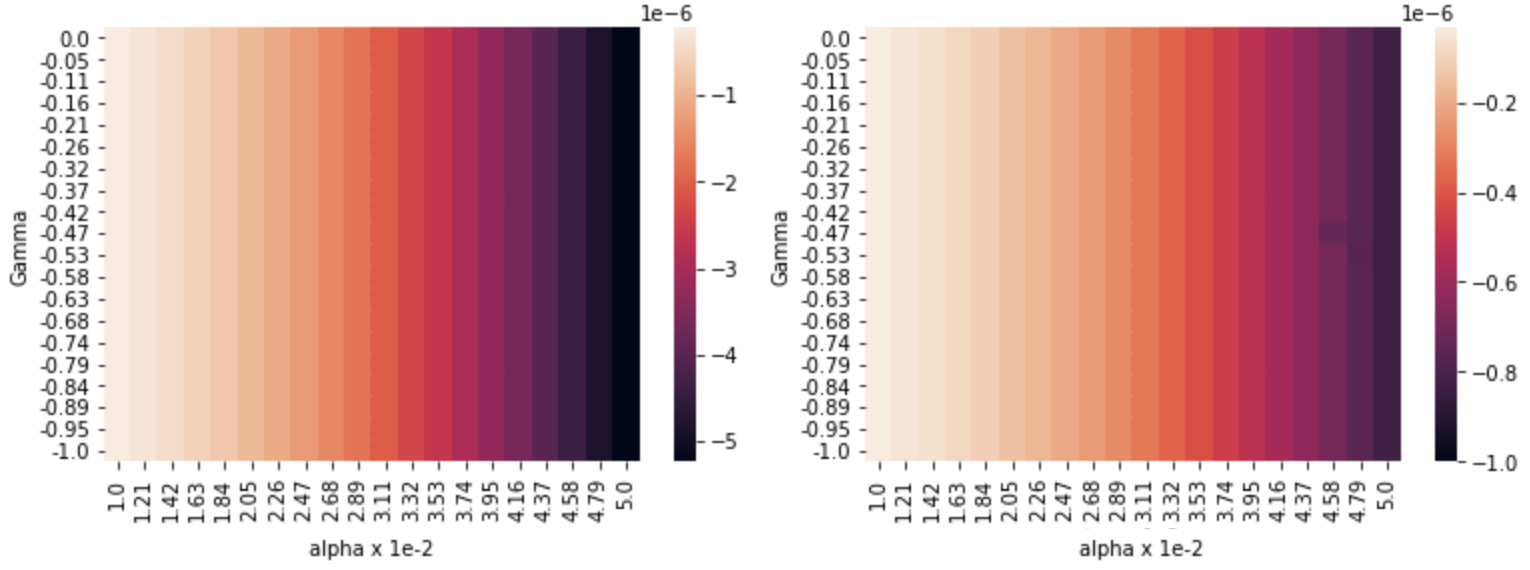
\includegraphics[width = 1.2 \linewidth, center]{Figures/Theory.png}
    \caption{Evaluation of (\ref{eqn::Final}) over a range of $\alpha$ and $\Gamma$ values. Lighter regions indicate where (\ref{eqn::Final}) is close to zero (i.e. close to the stability boundary) whilst darker regions are further away. We vary $\alpha$ in the range $[0.01, 0.05]$ and $\Gamma$ in the range $[-1, 0]$. $\tau = 0.05$. ( Left) $p = 2, N = 2$, (Right) $p = 3, N = 8$.}
    \label{fig:theory}
\end{figure}

%%% TO BE COMBINED WITH FIG 6

% \begin{figure}[t]
%     \centering
%     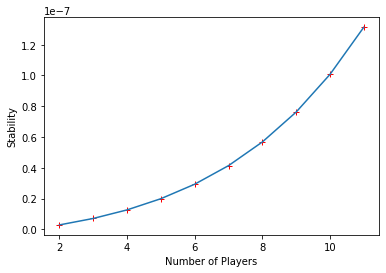
\includegraphics[width = .75\linewidth]{Figures/pVariance.png}
%     \caption{Evaluation of (\ref{eqn::Final}) for varying numbers of players $p$. Here, $\alpha$ is fixed at $0.02$, $\tau = 0.05$, $N = 2$ and $\Gamma = -1$. $p$ is varied from 2 to 12. We see that the value obtained by (\ref{eqn::Final}) tends away from zero monotonically.}
%     \label{fig:pvariation}
% \end{figure}

\textbf{Implication 5} can, as discussed, be seen directly from (\ref{eqn::Final}) itself. The prediction is that (\ref{eqn::Final}) will decrease (i.e. move away from the stability boundary) monotonically with $p$. This is due to the $(p - 1)$ term which appears in the equation.


%%%%%%%%%%%%% END THEORY %%%%%%%%%%%%%%%%%%%%%

%%%%%%%%%%%%% EXPT %%%%%%%%%%%%%%%%%%%%%

\section{Experimental Evaluation} \label{sec::exev}

As mentioned, the analytic result (\ref{eqn::Final}) holds in the limit of a large number of players and an infinite number of actions. It is therefore prudent to assess whether Implications 2--5 hold for games which are not in this limit. In this section, we describe and discuss the numerical experiments to verify the implications in Sec.~\ref{sec::discussion}. We first describe how these experiments were conducted, and then
%having presented the results in Figures \ref{fig:NumericalExperiments} and \ref{fig:pVarianceExpt}, 
we discuss the correlation with the theory.

\subsection{Construction of Numerical Experiments}

To verify experimentally the theoretical results, and to examine the underlying structure of stability and chaos in
multi-agent Q-learning, we perform a series of numerical experiments by varying the parameters $\Gamma$ and
$\alpha$, whilst keeping $\tau$ fixed. The aim is to determine the regions in which games learnt using Q-learning converge to an equilibrium. The results of these experiments are shown in Fig.~\ref{fig:NumericalExperiments}, with parameters chosen to match those in the analytic assessment (Fig.~\ref{fig:theory}).

To generate the numerical simulations in Fig.~\ref{fig:NumericalExperiments} we used the
following procedure.

\begin{enumerate}
   \item Fix the parameters $\tau$ and $\gamma$. The former is held at 0.05 and the latter at 0.1.
   \item Initialise values of $\Gamma$ and $\alpha$. These will be swept over in the experiment.
\item Generate 15 payoff matrices by sampling from a multi-variate Gaussian 
(variables are the payoff elements) with mean zero and covariance parameterised by $\Gamma$.
\item For each of these payoff matrices, initialise a set of agents with random initial conditions (i.e., random action probabilities).
\item Allow both sets of agents to learn over a maximum of $5 \times 10^4$ iterations.
\item Keep track of the action probabilities over a window of 5000 iterations. At the end of each window, determine the percentage difference between the maximum and minimum values of each strategy component.
\item If the difference is less than 1\% consider the game converged. Otherwise continue to the next window.
\item If the game reaches $5 \times 10^4$ iterations without satisfying the relative distance criterion, consider it to be non-convergent. Determine the fraction of these 15 games which have converged.

\end{enumerate}
  
We see in Fig.~\ref{fig:NumericalExperiments} that the stability of the system is highly dependent on
the value of $\alpha$ and $\tau$, but not on $\Gamma$.
  \begin{center}
      \begin{figure}[t]
            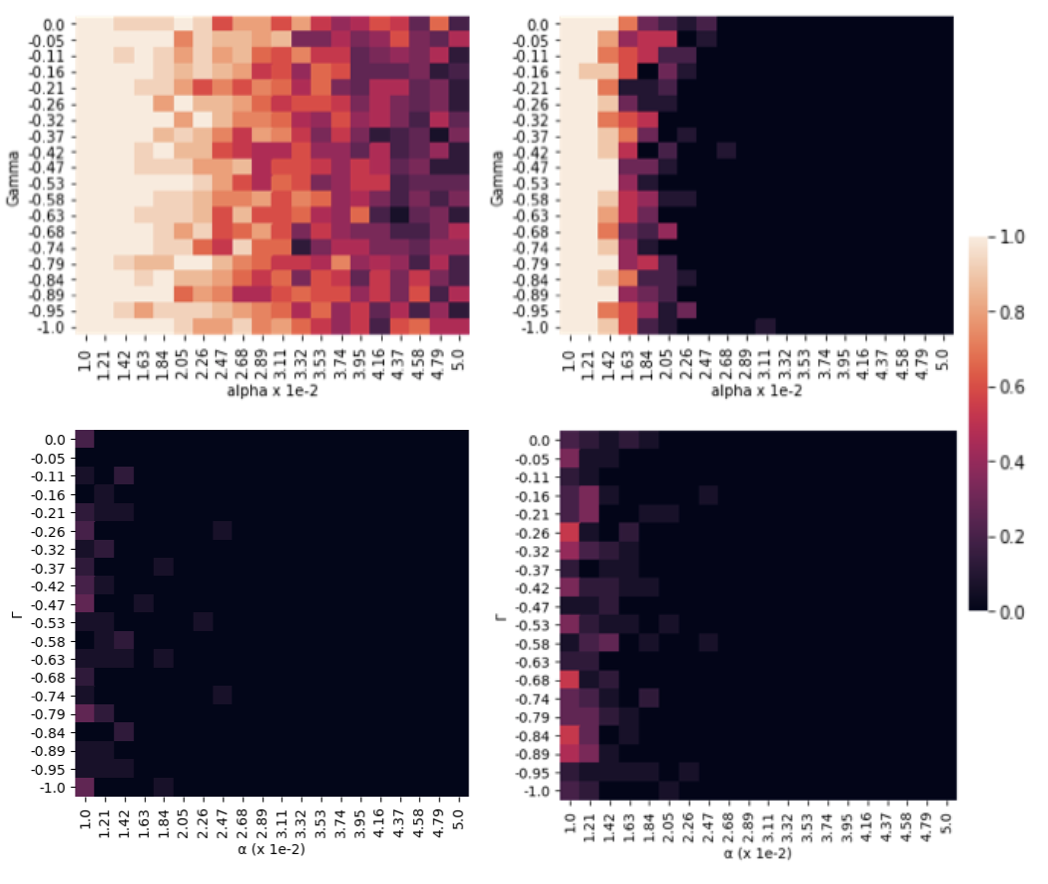
\includegraphics[width = 1.2 \linewidth, center]{Figures/Experiments.png}
            \caption{Results of numerical experiments in which $\alpha$ is varied. The heatmaps show the fraction of games which converge to an equilibrium. Lighter values show higher convergence. Each experiment is run with $\tau = 0.05$. (Top Left) $p = 2, N = 2$, (Top Right) $p = 2, N = 5$, (Bottom Left) $p = 3, N = 5$, (Bottom Right) $p=3, N = 8$.}
            \label{fig:NumericalExperiments}
        \end{figure}
  \end{center}


% \begin{figure}[t]
%     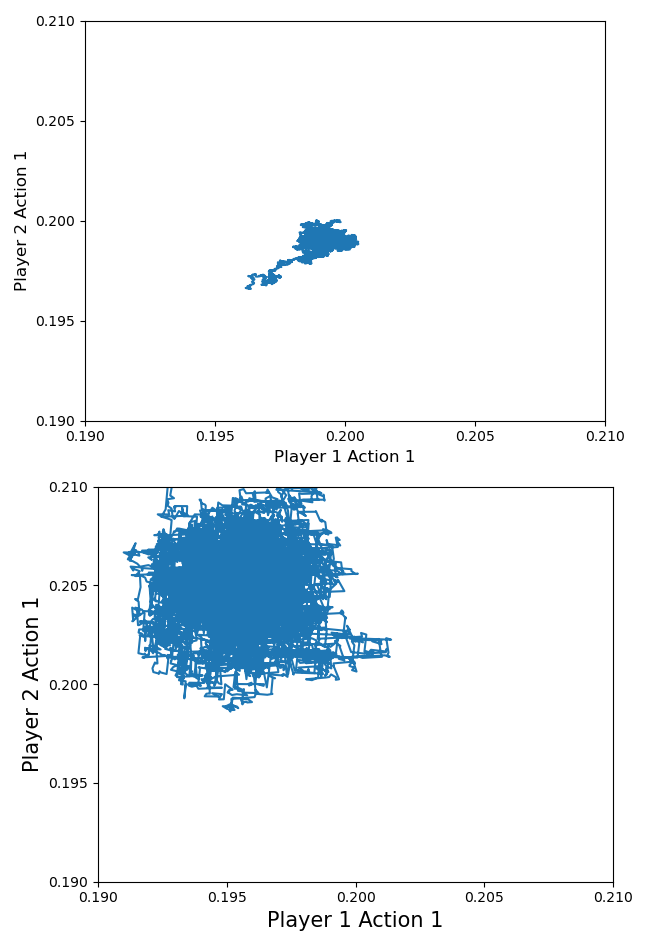
\includegraphics[width = 1.1 \linewidth, center]{Figures/alphavar5e2.png}
%     \caption{The trajectories of action probabilities for 2 players with 5 actions trained on a game of $\Gamma = -0.5$ and $\tau = 0.05$. (Left) $\alpha = 0.01$, (Right) $\alpha = 0.05$.}
%     \label{fig:AlphaVariation}
% \end{figure}



\begin{figure}[t]
    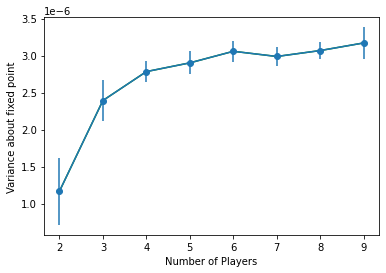
\includegraphics[width = .9\linewidth, center]{Figures/pVarianceExpt.png}
    \caption{Variation $V(t)$ about a fixed point as $p$ ranges from 2 - 9. $N = 2$, $\alpha = 0.02$, $\tau = 0.05$, $\Gamma \in [-1, 0]$. The experiment is conducted for 10 choices of $\Gamma$ and the mean (line) is plotted alongside the standard deviation (vertical bars).}
    \label{fig:pVarianceExpt}
\end{figure}

Finally, in Fig.~\ref{fig:pVarianceExpt} we plot the degree variation about the fixed point displayed as the number of players $p$ increases. The variation is determined by first allowing the game to iterate for 5000 steps, so that it can be assumed to have reached the vicinity of the fixed point. Then, the action probabilities are recorded for a further 5000 iterations. At the end of this second period, the variance of the actions is calculated as
%
\begin{equation*}
    V(t) = \frac{1}{N} \sum_i \big ( \frac{1}{5000} \sum_t x_i(t)^2 - \left[\frac{1}{5000} \sum_t x_i(t) \right]^2 \big ).
\end{equation*}

This gives a measure of the degree of variability about the fixed point and, therefore, gives some notion of the `degree of instability'.

Due to computational constraints, which we discuss in the following section, we are only able to increase $p$ to a maximum value of 9 . We maintain $\alpha = 0.02$ and $\tau = 0.05$. Finally, in Fig.~\ref{fig:pVarianceExpt}, we are averaging over 10 choices of $\Gamma$ in the range $[-1, 0]$. 

\subsection{Discussion}
    
We observe that the numerical experiments confirm the predictions
suggested by the analytic results in Fig.~\ref{sec::Theory}. We notice that convergence occurs almost only for
low values of $\alpha$. This observation stands as we increase the
number $N$ of actions. As noted in Sec. \ref{sec::discussion}, the analytic result over-estimates the region
of instability due to the assumptions $N \rightarrow \infty$ and
$\frac{1}{p-1} \ll 2$ made during the derivation. Remaining
discrepancies are due to the aforementioned approximation in
the calculation of $q$, $\chi$ and the fact that the analytic result
considers a continuous time approximation of the expected behaviour of
Q-learning. We expect that testing over a greater number of payoff
realisations and initial conditions will yield a more representative
assessment of the average behaviour of Q-learning. However, running
these experiments is a computationally expensive procedure: for $p$
players and $N$ actions we require operations on $p$ matrices with
$N^{p}$ elements. As such, due to a reduced availability of
computational facilities, a large scale averaging was not possible.

A key point which we wish to discuss here is a comparison with the result
found in~\cite{sanders:prevalence}, which considers the stability of
\textit{experience weighted attraction} (EWA). Namely, Sanders et
al.~observe that convergence is seen for higher values of $\alpha$,
whereas lower values give rise to chaos, the opposite of what is found
here. The reason for this can be seen in the update equation
(\ref{eqn::Qupdate}) for Q-learning, whereby smaller values of
$\alpha$ result in the agent placing a lower weight on the reward
received at each step. As such, lower values of $\alpha$ result in the
agent taking more conservative steps and yields a higher probability
of convergence. In contrast, the update for EWA does not discount the
reward received and, instead, only discounts the previous
knowledge of the Q-value based on higher choices of $\alpha$.  This
highlights the importance of performing analyses such as the present
work; it allows for a method to analytically compare the differences
between learning algorithms and, for practitioners, to ensure that the
appropriate algorithm is chosen for the parameters of their specific
task.

To summarise, we have shown that the analytic result
(\ref{eqn::Final}) provides a strong assessment of the effects that
parameters $\alpha$, $\tau$, $\Gamma$, and $p$ have on the likelihood of
convergence of Q-learning. Furthermore, though
(\ref{eqn::Final}) overestimates the region of instability by assuming $N \rightarrow \infty$, it
accurately conveys that convergence of Q-learning is increasingly unlikely for
games with many players and actions. In fact, our experimental results
also verify that stability may only be guaranteed for the limiting
case of two-player, two-action games.
%

\section{Conclusion}

In this study, we made a first contribution towards the
characterisation of the behaviours of agents learning how to play
$p$-player, $N$-action games through Q-learning. To this end, we
analysed the replicator model of Q-learning derived in \cite{tuyls:iteratedgames}. Specifically, we searched for the regions in parameter space
where the dynamics are expected to converge to a stable equilibrium
and those where learning is unstable. This yielded a number of
important results. We showed that for negatively correlated payoff matrices, the
strength of correlation $\Gamma$ does not influence stability; whereas, as
$\alpha$ and $\tau$ increase, the likelihood of convergence decreases. This behaviour differs from the stability of EWA, suggesting that different learning methods produce different qualitative behaviours. Similarly to EWA, however our
analysis also shows that the likelihood of convergence decreases,
regardless of parameter choice as the number of players $p$ in the
system increases.

As research into the dynamics of RL algorithms
progresses, it would be prudent to apply this analysis to various
other algorithm. Algorithms whose dynamics are established, and are
therefore open to a stability analysis, include piecewise Q-Learning
and Cross Learning. This would provide a strong method by which to
compare and provide safety guarantees to different algorithms for a
particular use case.

%%%%%%%%%%%%%%%%%%%%%%%%%%%%%%%%%%%%%%%%%%%%%%%%%%%%%%%%%%%%%%%%%%%%%%%%

%% The file named.bst is a bibliography style file for BibTeX 0.99c
\bibliographystyle{named}
\bibliography{references}

\end{document}